\subsection{\textcolor{red}{If nuclear energy can solve climate change, where
are all the reactors?}}


% \begin{enumerate}
% \item What do proponents of nuclear energy say about nuclear power?
% \begin{itemize}
%     \item Nuclear engineers generally understand that discomfort and fear around
%     nuclear power come from fears about nuclear weapons and fears about
%     radiation. As such, they view these fears as irrational and placatable by
%     "educating" and ignorant public.
%     \item Some general benefits of nuclear energy (high energy density, low
%     material requirements, low carbon footprint, "safe," low land requirements,
%     reliable, "resilient").
%     \item Additionally, advocates for nuclear energy point to the sustainability
%     of nuclear energy due to its high energy density which in turn reduces the
%     amount of harmful externalities associated with its fuel cycle, relative to
%     other technologies.
%     \item Finally, the nuclear industry has a clear understanding of its fuel
%     cycle, the ways nuclear materials may be reused and/or disposed of, and the
%     measures needed to ensure its safety.
% \end{itemize}
% \item What are the technical objections to nuclear?
% \begin{itemize}
%     \item Nuclear accidents
%     \item Waste (high level waste is a tremendous issue.)
%     \item Ethical issues around mining (what historical harms have been done to
%     mining communities? What about sourcing uranium from places like Kazakhstan
%     (allied to Russia) and directly funding the invasion of Ukraine? What
%     reparations have been made to those harmed? How will future harms be
%     prevented?)
%     \item Nuclear weapons proliferation (discuss the relationship between
%     nuclear energy and nuclear power. Additionally, although nuclear power
%     doesn't necessarily lead to weapons programs, the need to keep careful track
%     of nuclear materials and prevent its release into the biosphere, malicious
%     or otherwise, presents a profound responsibility with some intergenerational
%     inequities).
%     \item Nuclear energy is expensive.
% \end{itemize}
% \item What are some non-technical critiques of nuclear power?
% \item Why are engineering solutions insufficient?
% \begin{itemize}
%     \item Case study on yucca mountain + sweden + finland
%     \item Are advanced reactors actually being designed in a way that
%     incorporates people's preferences. Perhaps preferences toward nuclear energy
%     are not so dependent on the probability of an accident, but on the trust
%     between reactor owners and host communities. Non-experts don't have the
%     expertise to assess the importance of neutron spectra, fuel form, or other
%     technical design parameters that are important for safety. Asserting a low
%     accident probability does not inspire trust. If the reactor is so safe, why
%     not put your money where your mouth is (so-to-speak) and engage in profit
%     sharing with the community? ``Communities are not the final arbiters of
%     safety, determining safety is the purview of the Nuclear Regulatory
%     Commission.''


%     \textcolor{red}{Should I include a question about the benefit of
%     profit-sharing in human-subjects interviews? What are their concerns with
%     energy? Are they focused only on the production of energy or also the
%     lifecycle (extraction + disposal) as well?}
% \end{itemize}
% \end{enumerate}


%What do proponents of nuclear energy say about nuclear power?

In spite of its complicated history, nuclear energy has a variety of unique
benefits that researchers and advocates cite to support its continued and
expanded use. First, uranium has an enormous energy density. This fact has a
number of important consequences that favor the use of nuclear energy, such as
low land use \cite{lovering_land-use_2022,van_zalk_spatial_2018}, high \ac{eroi}
\cite{weisbach_energy_2013,murphy_energy_2022}, and a low mass and volume of
waste byproducts relative to other sources
\cite{liu_wind_2017,chowdhury_overview_2020,holdsworth_spent_2023,taebi_recycle_2008}.
Second, due to the nature of nuclear fission, nuclear power plants emit zero
carbon emissions, making them among the ``cleanest'' sources of energy along
with solar panels and wind turbines
\cite{nicholson_life_2021,intergovernmental_panel_on_climate_change_climate_2021,
brook_why_2014,van_de_graaff_understanding_2016}. Third, nuclear reactors
produce reliable baseload electricity and have the highest capacity factor of
any energy generating technology
\cite{brook_why_2014,van_de_graaff_understanding_2016}. Advocates for nuclear
energy also argue that nuclear energy is among the ``safest'' energy sources,
measured in deaths per unit energy produced
\cite{brook_why_2014,van_de_graaff_understanding_2016,sovacool_balancing_2016}.


%What are the technical objections to nuclear?
Although there are genuine benefits to producing electricity with nuclear
energy, concerns over its use persist. Nuclear engineers generally understand
that discomfort and fear around nuclear power come from fears about nuclear
weapons, nuclear plant accidents, and nuclear waste \cite{roeser_nuclear_2011}.
Each of these concerns are reflected in a different part of the nuclear fuel cycle,
shown in Figure \ref{fig:nuclear-fuel-cycle}.

\begin{figure}[ht]
    \centering
    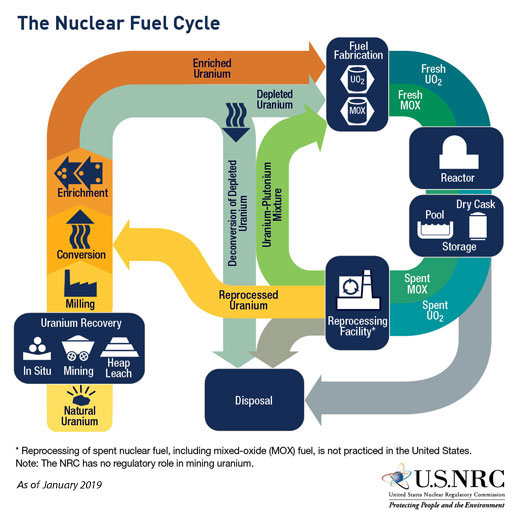
\includegraphics[width=0.5\columnwidth]{figures/nuclear-fuel-cycle-02.jpeg}
    \caption{Stages of the nuclear fuel cycle. Reproduced from \cite{nuclear_regulatory_commission_stages_2020}}
    \label{fig:nuclear-fuel-cycle}
\end{figure}

\noindent
Engineers typically adopt a ``hierarchical'' attitude, as described by cultural
theory of risk \cite{van_de_graaff_understanding_2016,mcneeley_cultural_2014},
and thus perceive these fears as irrational and placatable by ``educating'' an
ignorant public; consistent with the ``deficit model'' of science communication
\cite{simis_lure_2016,patenaude_topical_2022}. \textcolor{red}{It is incumbent
on nuclear engineers and advocates to adequately communicate the risks
associated with nuclear energy and not dismiss concerns due to a lack of
technical rigor.} Although \ac{snf} (commonly ``nuclear waste'') does not
present an immediate risk for radiological release, the details around managing \ac{snf} require
thoughtful consideration. Choosing between an open or a closed nuclear fuel
cycle implies different ethical foundations. Specifically, the tradeoff between
long- and short-term risks that must be carefully weighed
\cite{taebi_recycle_2008}. Further, even though civilian nuclear energy has not
led to the proliferation of nuclear weapons
\cite{herzog_nuclear_2020,miller_why_2017}, the need to keep careful track of
nuclear materials and prevent its release into the biosphere, malicious or
otherwise, presents a profound responsibility with some intergenerational
inequities. Finally, there are elements of the nuclear fuel cycle that 
are frequently ignored. In particular, mining and fuel fabrication are 
often overlooked by advocates for nuclear energy, even though mismanagement in these parts of
the nuclear fuel cycle have led to significant environmental disasters, such as the 
accident in Church Rock, New Mexico \cite{moore-nall_legacy_2015,rojavin_civilian_2011}. 

In addition to these ethical and technical issues, some have argued that, due to the
risks discussed above, nuclear energy requires centralized and authoritarian decision-making
structures and is therefore anathema to inclusive and democratic
values \cite{van_de_graaff_understanding_2016, winner_artifacts_1980}. However, conversations
within the nuclear spaces have reopened this question about the implicit ``politics'' of nuclear
energy, spurred on by the development of \acp{smr} \cite{lovering_social_2021}.

Distinct from conversations surrounding the ethics and risks of using nuclear
energy, many nuclear energy skeptics insist that nuclear power is too expensive
to support decarbonization goals. While it is true that nuclear power plants
have significant capital costs \cite{nrel_2020_2020} which have grown in many
countries due to additional regulations and safety requirements (i.e.,
``negative learning'') \cite{lovering_historical_2016}, it remains unclear
whether these costs uniquely translate to burden on electricity consumers.
Especially given nuclear energy's role as a ``price-taker'' in electricity
markets \cite{murphy_impacts_2019} and evidence for nuclear's stabilizing effect
on electricity prices \cite{dotson_influence_2022,de_sisternes_value_2016}.

